%\renewcommand{\captionfont}{\textit}
\documentclass[twocolumn,twoside,slac]{revtex4}
%\setlength{\voffset}{-1.54cm}
%\setlength{\hoffset}{-0.54cm}
%\setlength{\evensidemargin}{1.5cm}
%\setlength{\marginparsep}{0cm}
%\setlength{\textwidth}{15cm}
%\setlength{\textheight}{24.7cm}
%\setlength{\topmargin}{1cm}
%\setlength{\headheight}{0pt}
%\setlength{\headsep}{0pt}

% The path of picture directory is described in the environmental string
%   ($LAWPICSPATH)
% The name and path of the BiBTeX bibliography file is defined in
%   ($LAWBIBNAME)

%\usepackage{epsf}
\usepackage{graphicx}
\usepackage{makeidx}
\usepackage{fancyhdr}

%\fancypagestyle{lawbody}{
%  \renewcommand{\headrulewidth}{0.5pt}
%  \fancyhead[LE,LO]{SiBT DAQ article / draft v0.13 (\input{draft.timestamp})}
%  \fancyhead[RE,RO]{Comments to lauri.wendland@cern.ch}
%  \fancyfoot[CE,CO]{\thepage}
%}

\pagestyle{fancy}
\fancyhead{} % clear all fields
\fancyhead[C]{\it {CHEP 2003, La Jolla, California, March 24-28 2003}} 
%{\bf (draft v1.05 \input{draft.timestamp})}
\fancyhead[RO,LE]{\thepage}
\fancyfoot{} % clear all fields
\fancyfoot[LE,LO]{\bf TUGP006}
\renewcommand{\headrulewidth}{0pt}
\renewcommand{\footrulewidth}{0pt}
\renewcommand{\sfdefault}{phv}

\setlength{\textheight}{235mm}
\setlength{\textwidth}{170mm}
\setlength{\topmargin}{-20mm}


% You should use BibTeX and apsrev.bst for references

\bibliographystyle{apsrev}

\begin{document}


%------------------------------< HEADER >------------------------------
\title{Bertini intra-nuclear cascade implementation in Geant4}

\author{Aatos Heikkinen, Nikita Stepanov} 
\affiliation{Helsinki Institute of Physics, P.O. Box 64, FIN-00014
  University of Helsinki, Finland}

%\author{Nikita Stepanov}
%\affiliation{:::}

\author{Johannes Peter Wellisch}
\affiliation{CERN}
%-----------------------------< ABSTRACT >-----------------------------
\begin{abstract}

We present here a intra-nuclear cascade model implemented in Geant4 5.0. 
The cascade model is based on re-engineering of INUCL code.
Models included are Bertini intra-nuclear cascade model with exitons, pre-equilibrium model, nucleus explosion model, 
fission model, and evaporation model.
Intermediate energy nuclear reactions from 100~MeV to 3~GeV energy are treated for proton, neutron, pions, photon and nuclear isotopes.
We represent overview of the models, review results achived from simulations and make comparisons with experimental data.

\end{abstract}

%\maketitle must follow title, authors, abstract
\maketitle

\thispagestyle{fancy}

% body of paper here - Use proper section commands
% References should be done using the \cite, \ref, and \label commands
% Put \label in argument of \section for cross-referencing
%\section{\label{}}


\section{INTRODUCTION}

The intra-nuclear cascade model (INC) was first proposed by Serber in 1947 \cite{serber47}.  
He noticed that, in particle-nuclear collisions the deBroglie wavelenght of the incident particle is 
comparaple (or shorter) than the average intra-nucleon distance.
Hence, the justification for describing the interactions in terms of particle-particle  collisions.

The INC has been succesfully used in the Monte Carlo simulations at intermediate energy region 
since Goldberger made first calculations by hand in 1947 \cite{goldberger48}. 
First computer simulations were done by Metropolis et al. in 1958 \cite{metropolis58}. 
Standard methods in INC implementations were formed when Bertini published his results in 1968 \cite{bertini68}.
Important addition was exiton model itroduced by Griffin in 1966 \cite{griffin66}. 

Our presentations describes implementation of Bertini INC model in Geant4 hadronic physics framework \cite{geant4collaboration03}.
Geant4 is a Monte Carlo particle detector simulation toolkit, having applications also in  medical and space
science. 
Geant4 provides a flexible framework for the modular implementation of
various kinds of hadronic interactions. 
Geant4 exploits advanced Software Engineering techniques and Object
Oriented technology to achieve the transparency of the physics
implementation and to this way provide the possibility of validating the
physics results. 

The hadronic models framework is based on concepts of physics
processes and models. While the process is a general concept, models
are allowed to have restrictions in process type, material, element
and energy range.  Several models can be utilized by one model class; for instance, a
process class for inelastic collisions can use distinct models for different energies.


Process classes utilize model classes to determine the
secondaries produced in the interaction and to calculate the momenta
of the particles. Here we preset a collection of such models providing medium-energy
intra-nuclear cascade treatment.


\section{GEANT4 CASCADE MODEL}

In inelastic particle-nucleus collision a fast phase ($10^{-23} - 10^{-22} s$) of INC results to highly exited nucleus, 
and is followed possible by fission and pre-equilibrium emission. 
A slower ($10^{-18} - 10^{-16} s$) compound nucleus phase follows with evaporation.
A Boltzman equation must be solved to treat physical proces of collision in detail.
 
Intra-nuclear cascade model developed by Bertini \cite{bertini68, bertini69, bertini71}, solves the Boltzman equation on the average.
The model have been implemented in several codes such as HETC \cite{alsmiller90}. 
Our model is based on re-engineering of INUCL code \cite{titarenko99a}.
Models included are Bertini intra-nuclear cascade model with exitons, pre-equilibrium model, simple nucleus explosion model, fission model, and evaporation model. 

Nuclear model consist of a three-region approximation to the continuously changing density distribution of nuclear matter within nuclei.
Reletivistic kinematics is applied throughout the cascade.
Cascade is stopped when all the particles, which can escape the nucleus, do it. 
Then conformity with the energy conservation law is checked.


\subsection{Model limits}

Particles treated are proton, neutron, pions, photon and nuclear isotopes.
Bullet particle can be proton, neutron or  pion.
Range of targets allowed is arbitrary.

The necessary condition of validity of the INC model is $\lambda_{B} / v << \tau_{c} << \Delta t$, 
where $\lambda_{B}$ is the deBroglie wavelenth of the nucleons, 
v is the average relative nucleon-nucleon velocity and $\Delta t$ is the time interval between collisions.
So the physical foundation comes approximate at energies less than $200 MeV$, and needs to be supported with pre-quilibrium model.
Also, at energies higher than 5-10 GeV, the INC picture breaks down.
Our implementation in Geant4 has been tested with bullet kinetic energy between 100~MeV and 3~GeV.

\subsection{Intra-nuclear cascade model}

Basic steps of the INC model are summarised below:

\begin{enumerate}
\item The spatial point, where the incident particle enters, is selected uniformly over the projected area of the nucleus.
\item Total particle-particle cross-sections and region-depenent nucleon densities are used to select a path lenght for the projectile particle.
\item The momentum of the struck nucleon, the type of reaction and four momentum of the reaction products are determined.
\item Exiton model is updated as the cascade proceeds.
\item If Pauli exclusion principle allows and $E_{particle} > E_{cutoff}$ = 2~MeV, step (2) is performed to transport the products.
\end{enumerate}

After INC, the residual excitation energy of the resulting nucleus is used as input for non-equilibrium model. The scematic presentation of Bertini INC is visualized in Fig.~\ref{figMC}


\begin{figure}
  \includegraphics[width=80mm,keepaspectratio]{mc.eps}
  \caption{Schematical presentation of intra-nuclear cascade. A hadron with 400 MeV energy is forming INC. Crosses present the Pauli exclusion principle in action. (The picture is a reproduction from original work of Bertini \cite{bertini68}.)}
  \label{figMC}
\end{figure}



\subsection{Nuclei model}

Some of the basic features of the nuclei are:

\begin{itemize}
\item The nucleons are assumed to to have a Fermi gas momentum distribution. 
Fermi energy is calculated in a local density approximation i.e. 
Fermi energy is made radius dependent with Fermi momentum $p_{F}(r) = (\frac{3 \pi^2 \rho(r)}{2})^\frac{1}{3}$.
%\item Nuclear density effects are recalculated after each step.
\item Nucleons binding energies (BE) are calculated using mass formula.
A parametrization of the nuclear binding energy uses combination of Kummel mass formula, and
experimental data. Also, asymptotic high temperature mass formula is used, 
if it's impossible to use experimental data.
\end{itemize}

\subsubsection{Initialization}
The initialization phase fixes of nucleus radius  and momentum according to Fermi gas model.

If target is Hydrogen (A = 1), a direct particle-particle collision is performed, 
and no nuclear modelling is used. 


If $1 < A < 4$, a nuclei model consisting one layer with radius of 8.0 fm is created.


For $4 < A < 11$, a nuclei model is composed of three consentric spheres $i = \{1, 2, 3\}$ with radius
$$r_{i}(\alpha_{i}) = \sqrt{C_{1}^{2} (1 - \frac{1}{A}) + 6.4} \sqrt{-log( \alpha_{i})}$$

where $\alpha_{i} = \{0.01, 0.3, 0.7\}$ and $C_{1} = 3.3836 A^{1/3}$

If $A > 11$, nuclei model with three consentric spheres is also used. The shere radius is now defined as:
$$r_{i}(\alpha_{i}) =  C_{2} \log({\frac{1 + e^{- \frac{C_{1}}{C_{2}}}}{\alpha_{i}} - 1}) + C_{1}$$

where $C_{2} = 1.7234$.

The potential energy for nucleon N is
$$ V_{N} = \frac{p_{F}^2}{2 m_{N}} + BE_{N}(A, Z)$$

where $p_F$ is a Fermi momentum and BE a binding energy. 
 
Impulse distribution in each region follows Fermi distribution with zero temperature.

\begin{equation}
 f(p) = c p ^2
 \end{equation}

 where

 \begin{equation}
 \int_0^{p_F} f(p) dp = n_{p} \hspace{0.2truecm}  or \hspace{0.2truecm}   n_{n}
 \end{equation}

 where $n_p$ and $n_n$ are the number of protons or neutrons in region and 
$p_F$ is impulse corresponding the Fermi energy

 \begin{equation}
 E_F = \frac{p_F^2}{2 m_N} = \frac{\hbar^2}{2 m_N}(\frac{3 \pi^{2}}{v})^\frac{2}{3}
 \end{equation}
 
 which depend on the dencity $n/v$ of particles. 
 and which is different for each particle and each region. 

\subsubsection{Pauli exclusion principle}
Pauli exclusion principle forbids interactions where the products would be in occupied states.
Following an assumption of completely degenerate Fermi gas, the levels are filled from the lowest level.
The minimum energy allowed for the product of collision correspond to the lowest unfilled level of system, which is the Fermi energy in the region. 
So in practice, Pauli exclusion principle is taken into account by accepting only secondary nucleons which have $E_N > E_F$.


\subsubsection{Cross-sections and kinematics}

Path lengths of nucleons in the nucleus are sampled according to the local density and to free nucleon-nucleon cross-sections.
Angles after collisions are sampled from experimental differential cross-sections.
%Geant4 cascade model uses tabulated cross-sections.
Tabulated total reaction cross-sections are calculated by Letaw's formulation \cite{letaw83, letaw93, pearlstein89}.
%:::$45 A^0.7 (1+0.016 sin(5.3-2.63 log10(A)))^(1-0.62 exp(-E / 200) sin(10.9 E^(-0.28)))
For nucleon-nucleon cross-sections parametrizations based on the experimental energy and isospin dependent data. 
The parameterization described in \cite{barashenkov72} is used. 

For pion the INC cross-sections are provided to treat elestic collisions, and inelastic channels:
$\pi^{-}$n $\rightarrow$ $\pi^{0}$n, $\pi^{0}$p $\rightarrow$ $\pi^{+}$n and $\pi^{0}$n $\rightarrow$ $\pi^{-}$p.
Multiple particle production is also implemented.

Pion absorption cannels 
$\pi^{+}$nn $\rightarrow$ pn, $\pi^{+}$pn $\rightarrow$ pp, 
$\pi^{0}$nn $\rightarrow$ X , $\pi^{0}$pn $\rightarrow$ pn,      $\pi^{0}$pp $\rightarrow$ pp, 
$\pi^{-}$nn $\rightarrow$ X , $\pi^{-}$pn $\rightarrow$ nn , and $\pi^{-}$pp $\rightarrow$ pn are implemented.


\subsection{Pre-equilibrium model}

Geant4 cascade model implements exiton model proposed by Griffin \cite{griffin66}.
In his model nucleon states are characterized by the number of exited particles and holes (the exitons).
INC collisions give rise to a sequence of states characterized by increasing exciton number, eventually leading to a equilibrated nucleus.
For practical implementation of exiton model we use level density parameters from \cite{ribansky73} and  matrix elements from \cite{kalbach78}.

In exiton model the posible selection rules for a particle-hole configuarations in the cource of the cascade are:
$\Delta p = 0, \pm 1$  $\Delta h = 0, \pm 1$  $\Delta n = 0, \pm 2$,
where p is the number of particle, h is number of holes and n = p + h is the number of exitons. 

Cascade pre-equilibrium model uses target exitation data, 
exiton configuration for neutron and proton to produce non-equilibrium evaporation.
The angular distribution is isotropic in the frame of rest of the exiton system.

Parametrisations of the level density, is tabulated both with A and Z dependence and with high temperature 
behaviour. The nuclei binding energy is using smooth liquid high energy formula.

%N $\rightarrow$ N - 2, N $\rightarrow$ N - 1 N $\rightarrow$ N, N $\rightarrow$ N + 2,  channels are treated.

\subsection{Break-up models}


Fermi break-up is allowed only in some extreme cases, i.e. for light nuclei ($A < 12$ and  $3 (A - Z) < Z < 6$ ) and 
if $E_{exitation} > 3 E_{binding}$ .
Simple explosion model decays the nuleus into neutrons and protons and decreases exotic evaporation processes.

Fission model is phenomenological model using potential minimization. 
Binding energy paramerization is used and some features of the fission statistical model are incorporated \cite{fong69}.


\subsection{Evaporation model}

Statistical theory for particle emission of the exited nucleus remaining after the INC was originally developed by Weisskopf \cite{weisskopf37}. 
This model assumes complete energy equilibration before the particle emission, and re-equilibration of excitation energies between successive evaporations. 
As a result the angular distribution of emitted particles is isotropic.

Geant4 evaporation model for cascade implementation adapts often used computational method developed by Dostrowski \cite{dostrovsky59, dostrovsky60}.
The emission of particles is computed until the exitation energy fall below some spesific cutoff. 
If light nucleus is higly exited Fermi break-up model is executed. Also, fission is performed if channel is open. 
The main chain of evaporation is followed until  $E_{exitation}$ falls below E$_{cutoff}$ = 0.1 MeV. 
The evaporation model ends with  emission chain, which is followed until E$_{exitation}$ $<$ E$^{\gamma}_{cutoff}$ = 10$^{-15}$ MeV.

%Evaporation (Weisskopf - Ewing) 
%Weisskopf-Ewing evaporation in competition with fission. 

%line\cite{SiBT_hardware99, SiBT2000a}. It is used



\section{IMPLEMENTATION}

% \subsection{Geant4 hadronic framework}

Cascade model is implemented in Geant4 hadronic physics framework. (Bertini cascade source code module is located in directory {\it geant4/\-source/\-processes/\-hadronic/\-models/\-cascade/\-cascade}.)
All the models are used collectively through interface method {\it Apply\-Yourself} defined in a class {\it G4Cascade\-Inteface}.
A Geant4 track  ({\it G4Track}) and a nucleus ({\it G4Nucleus}) are given as a parameters.


Currently implementation is not optimized for speed.
The typical timing behaviour for different target nuclons and bullet energies is presented in Fig.~\ref{timingModel}.

\begin{figure}
  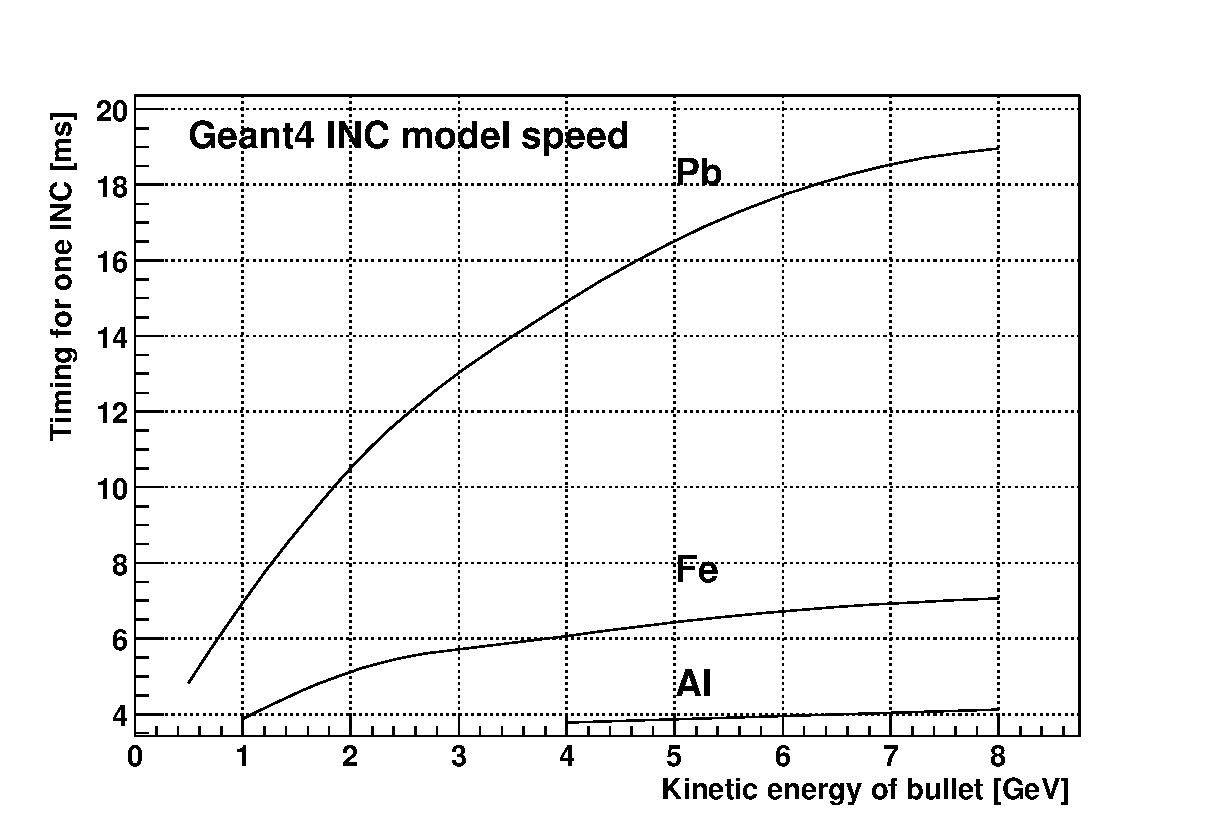
\includegraphics[width=80mm,keepaspectratio]{tIsotopeVsEnergy.eps}
  \caption{Speed of single INC performed for Al, Fe and Pb nuclei for proton bullet at energy-range 1-8 GeV.
A single PC with 300 MHz PII is used.}
  \label{timingModel}
\end{figure}

\section{RESULTS}
\label{results}

We have tested the physics performance of Bertini cascade models in a first Geant4 5.0 implementation, for energies 100~MeV -- 3~GeV. 
Detailed comparisons with experimental data has been made in energy range 160 -- 800 MeV.
 

A double differential cross-sections for neutrons at $7.5^{\circ}$, $30^{\circ}$, $60^{\circ}$, and $150^{\circ}$ angles are presented in Figs.~\ref{n7}-\ref{n150} respectively. Proton bullet particle at 256 MeV energy is hitting iron target and all Bertini submodels are used.

%in Fig.~\ref{pbN60} and Fig.~\ref{pbPi60}.


\begin{figure}
  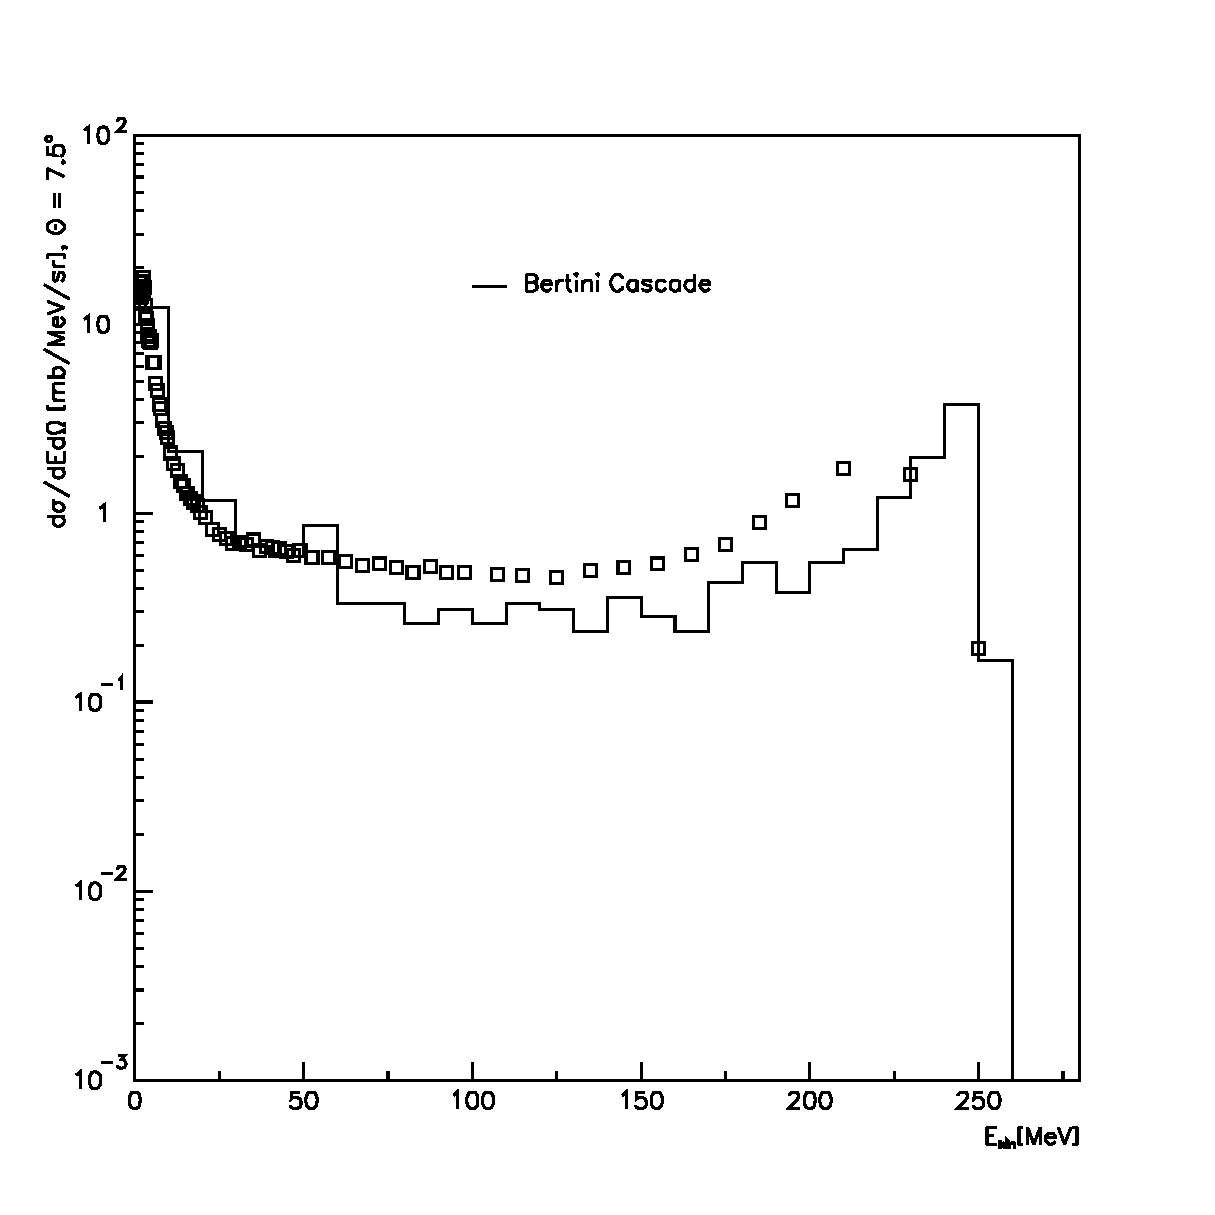
\includegraphics[width=80mm, keepaspectratio]{pn_fe_256_n_a0.eps}
  \caption{Geant4 Bertini INC model simulation of $p(256 MeV)$ + Fe $\rightarrow$ $n(\theta = 7.5^{\circ})$ + X in comparison with experimental data \cite{benchmarkData02}.}
  \label{n7}
\end{figure}

\begin{figure}
  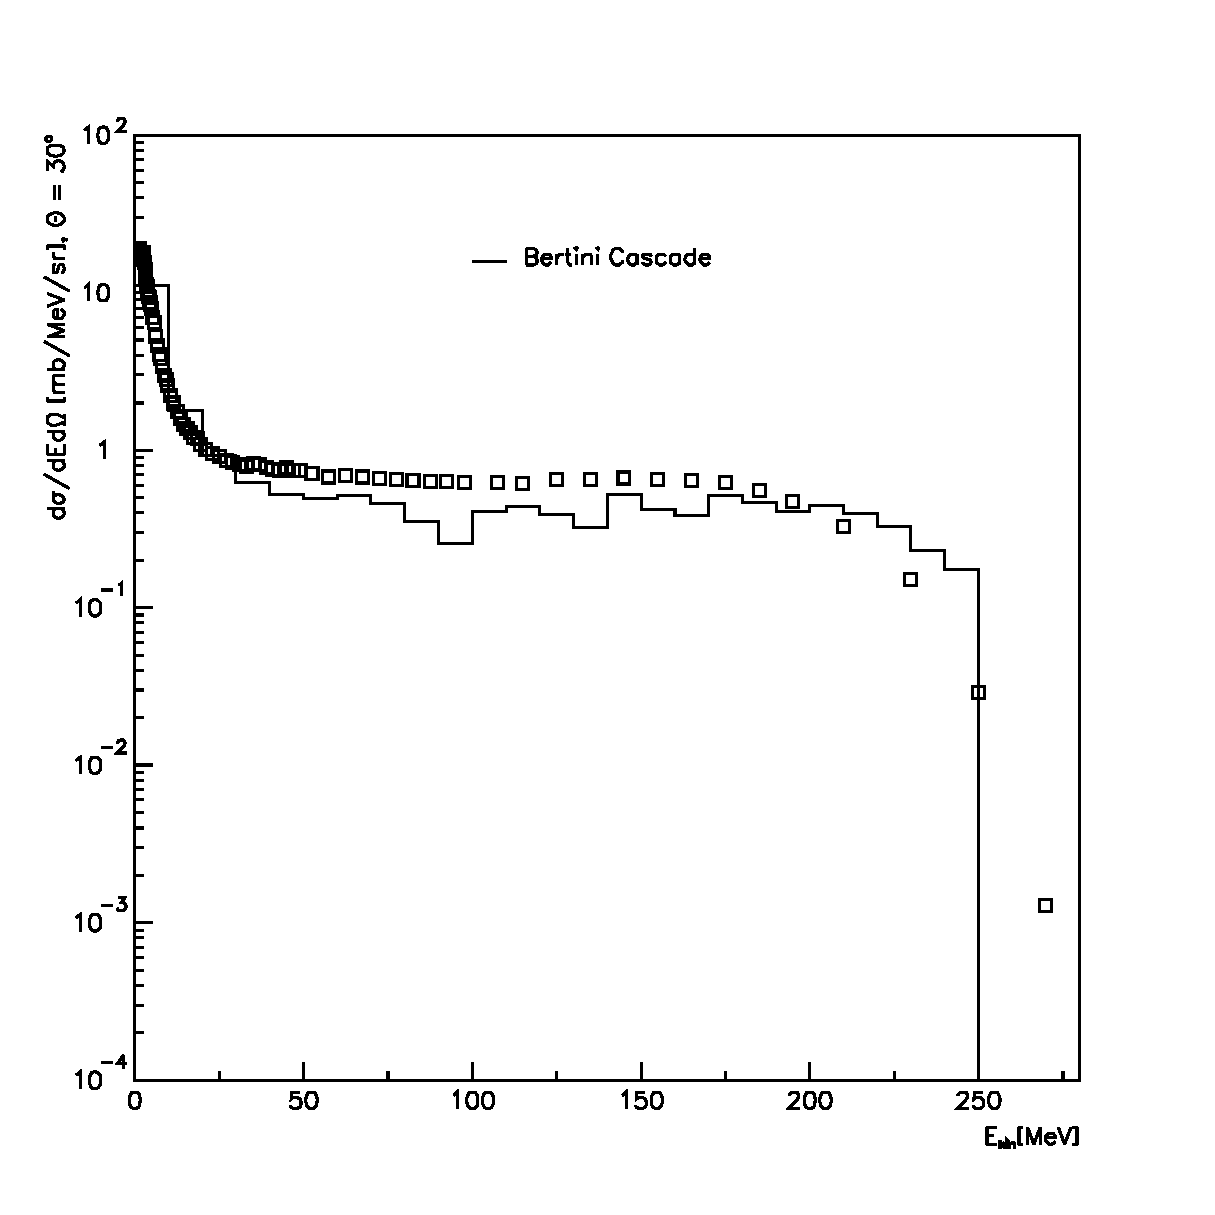
\includegraphics[width=80mm,keepaspectratio]{pn_fe_256_n_a1.eps}
  \caption{$p(256 MeV)$ + Fe $\rightarrow$ $n(\theta = 30^{\circ})$ + X.}
  \label{n30}
\end{figure}

\begin{figure}
  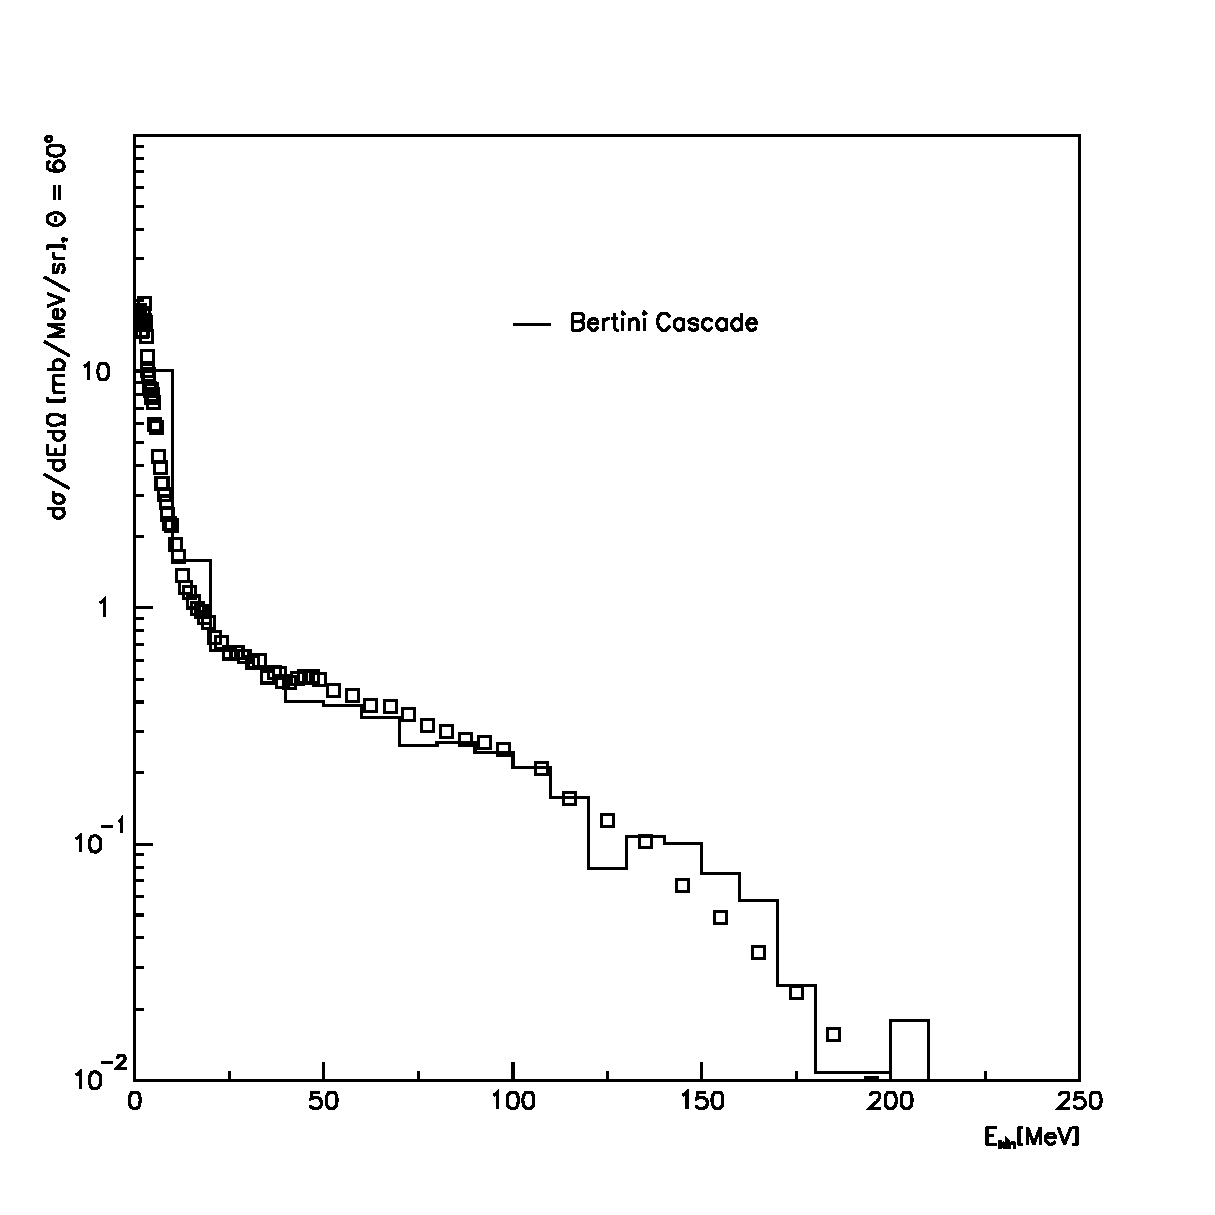
\includegraphics[width=80mm,keepaspectratio]{pn_fe_256_n_a2.eps}
  \caption{$p(256 MeV)$ + Fe $\rightarrow$ $n(\theta = 60^{\circ})$ + X.}
  \label{n60}
\end{figure}


\begin{figure}
  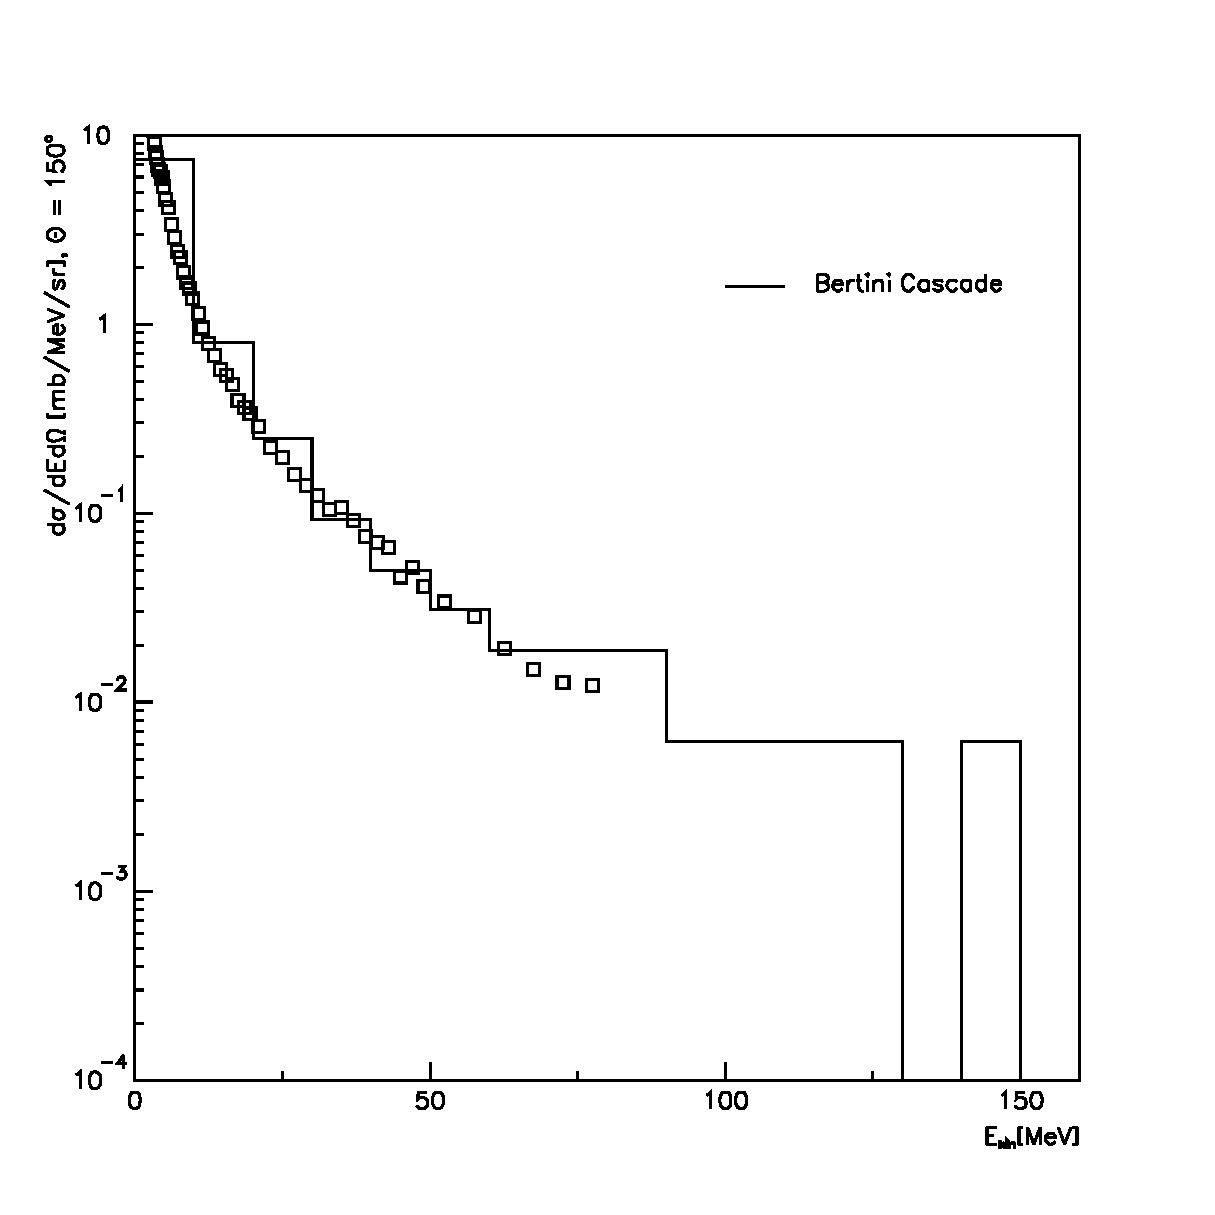
\includegraphics[width=80mm,keepaspectratio]{pn_fe_256_n_a4.eps}
  \caption{$p(256 MeV)$ + Fe $\rightarrow$ $n(\theta = 150^{\circ})$ + X.}
  \label{n150}
\end{figure}


%--------------------


Figures \ref{pbn60} and \ref{pbn120} show double differential cross-section of neutrons resulting from 597 MeV proton targeting lead. 

\begin{figure}
  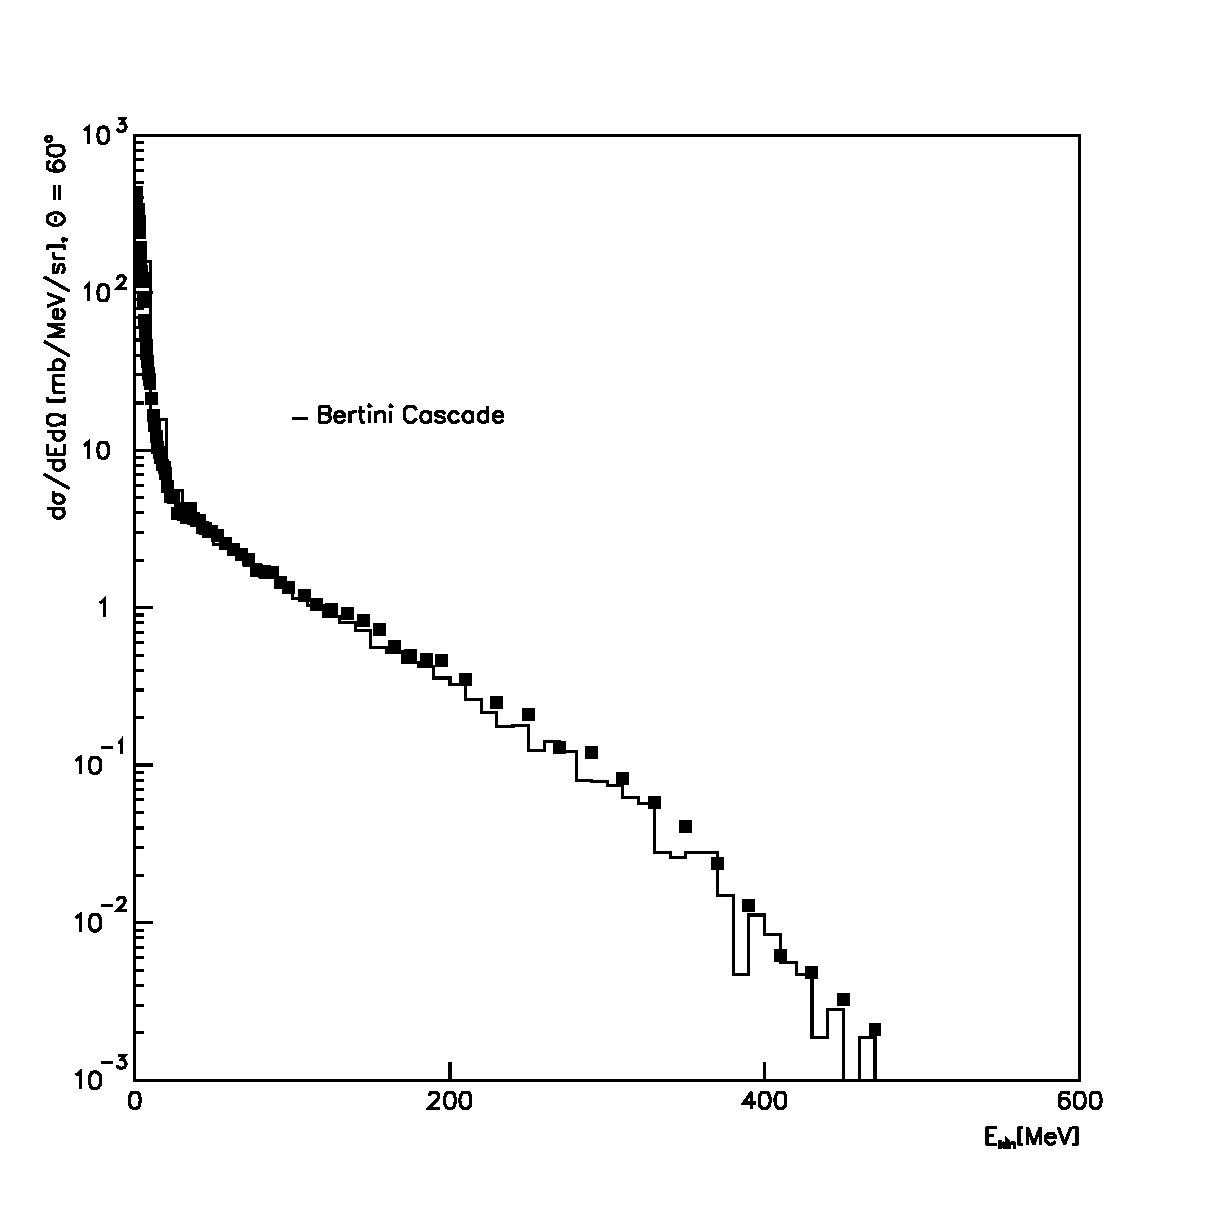
\includegraphics[width=80mm,keepaspectratio]{pn_pb_597_n_a1.eps}
  \caption{Geant4 Bertini INC model simulation of 
$p(597 MeV)$ + Pb $\rightarrow$ $n(\theta = 60^{\circ})$ + X 
in comparison with experimental data \cite{benchmarkData02}.}
  \label{pbn60}
\end{figure}


\begin{figure}
  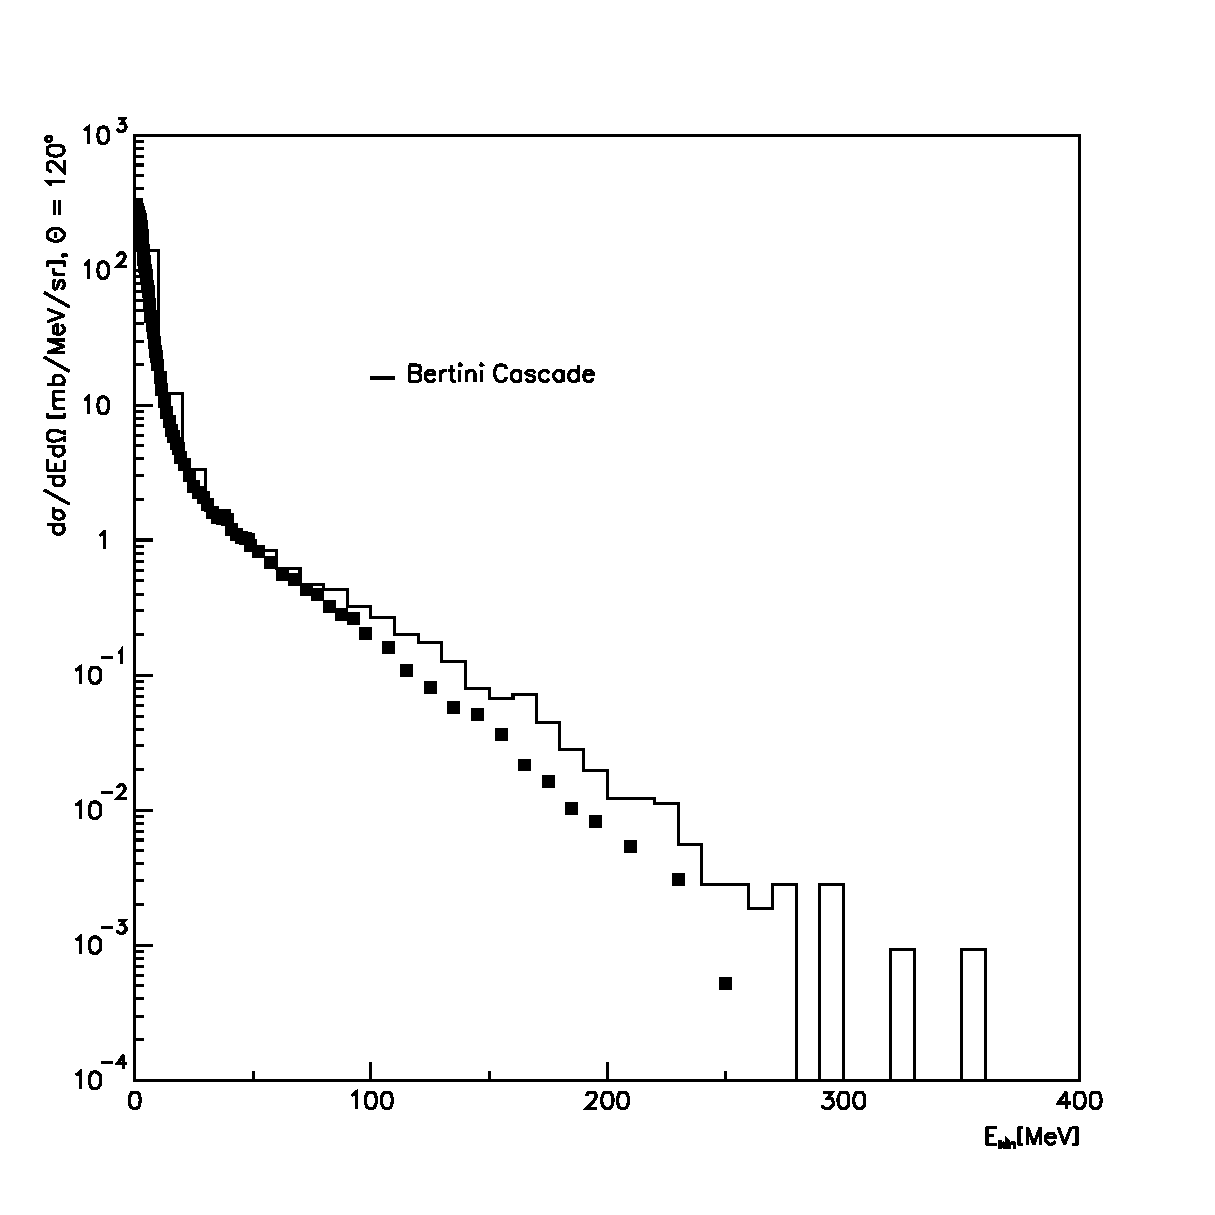
\includegraphics[width=80mm,keepaspectratio]{pn_pb_597_n_a3.eps}
  \caption{$p(597 MeV)$ + Pb $\rightarrow$ $n(\theta = 120^{\circ})$ + X.}
  \label{pbn120}
\end{figure}

%----------------------------



Finally, an example of pion production physics performace.
Double differential cross-sections for $\pi^{+}$ are given for
angels from $22.5^{\circ}$ to $135^{\circ}$ in Figs.~\ref{pi22}-\ref{pi135}.
%angels $22.5^{\circ}$, $45^{\circ}$, $60^{\circ}$, $^135{\circ}$ in Figs.~\ref{pi22}-\ref{pi135}.


An agreement with experimental data is found to be from moderate to relatively good.

 
\begin{figure}
  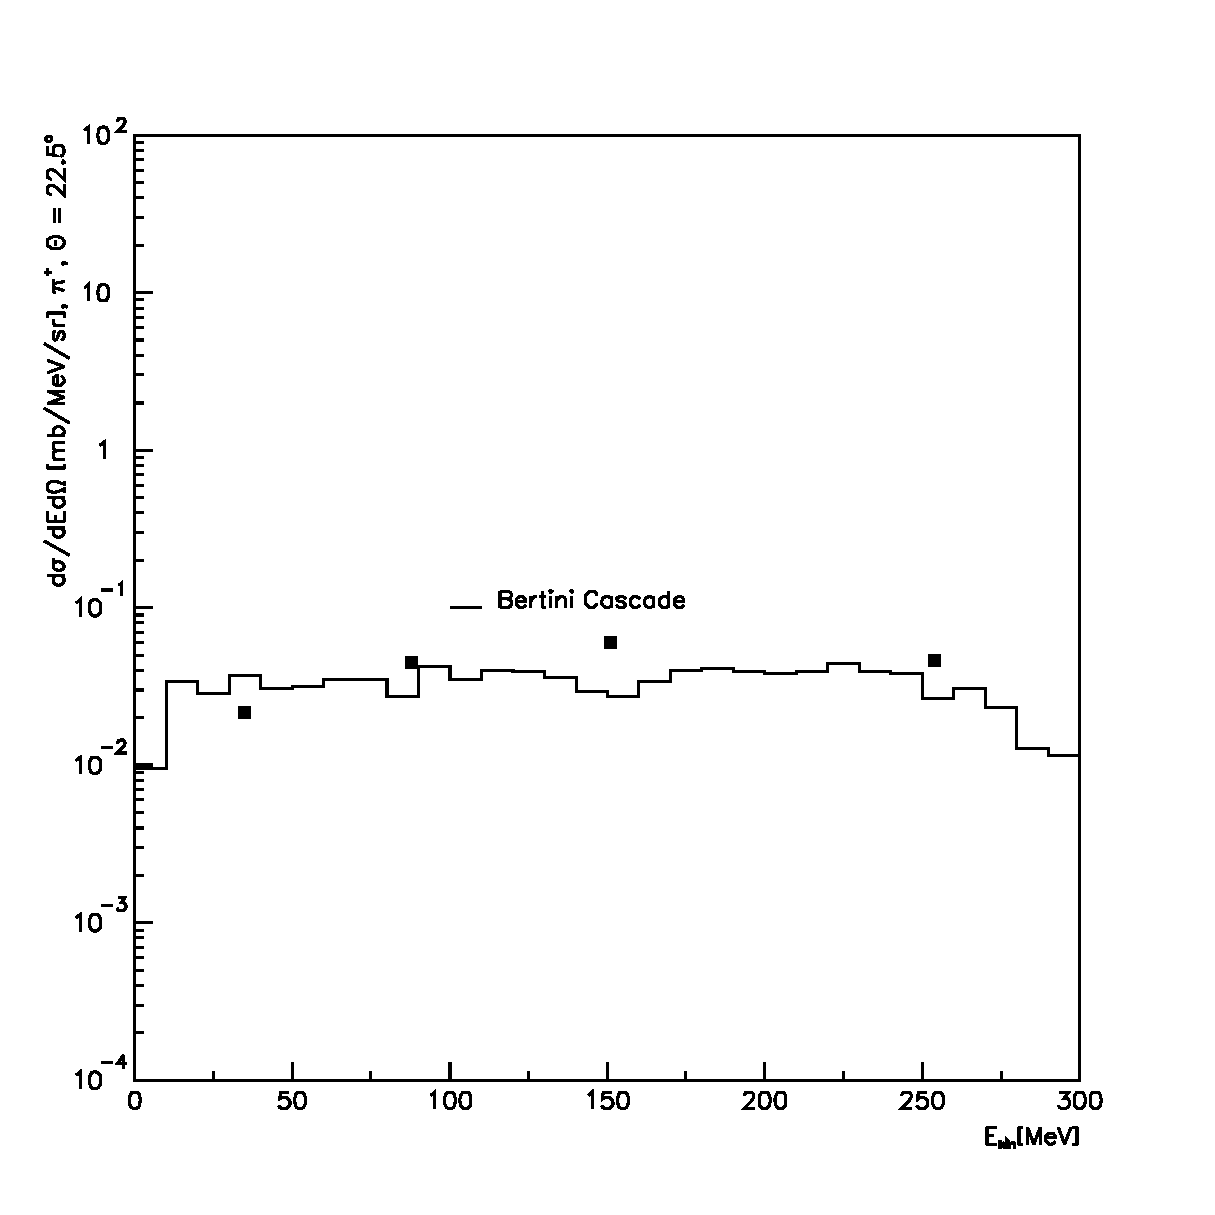
\includegraphics[width=80mm,keepaspectratio]{pn_pb_597_pip_a0.eps}
  \caption{Geant4 Bertini INC model simulation of
$p(597 MeV)$ + Pb $\rightarrow$ $\pi^{+}(\theta = 22.5^{\circ})$ + X
in comparison with experimental data \cite{benchmarkData02}.}
  \label{pi22}
\end{figure}
 

\begin{figure}
  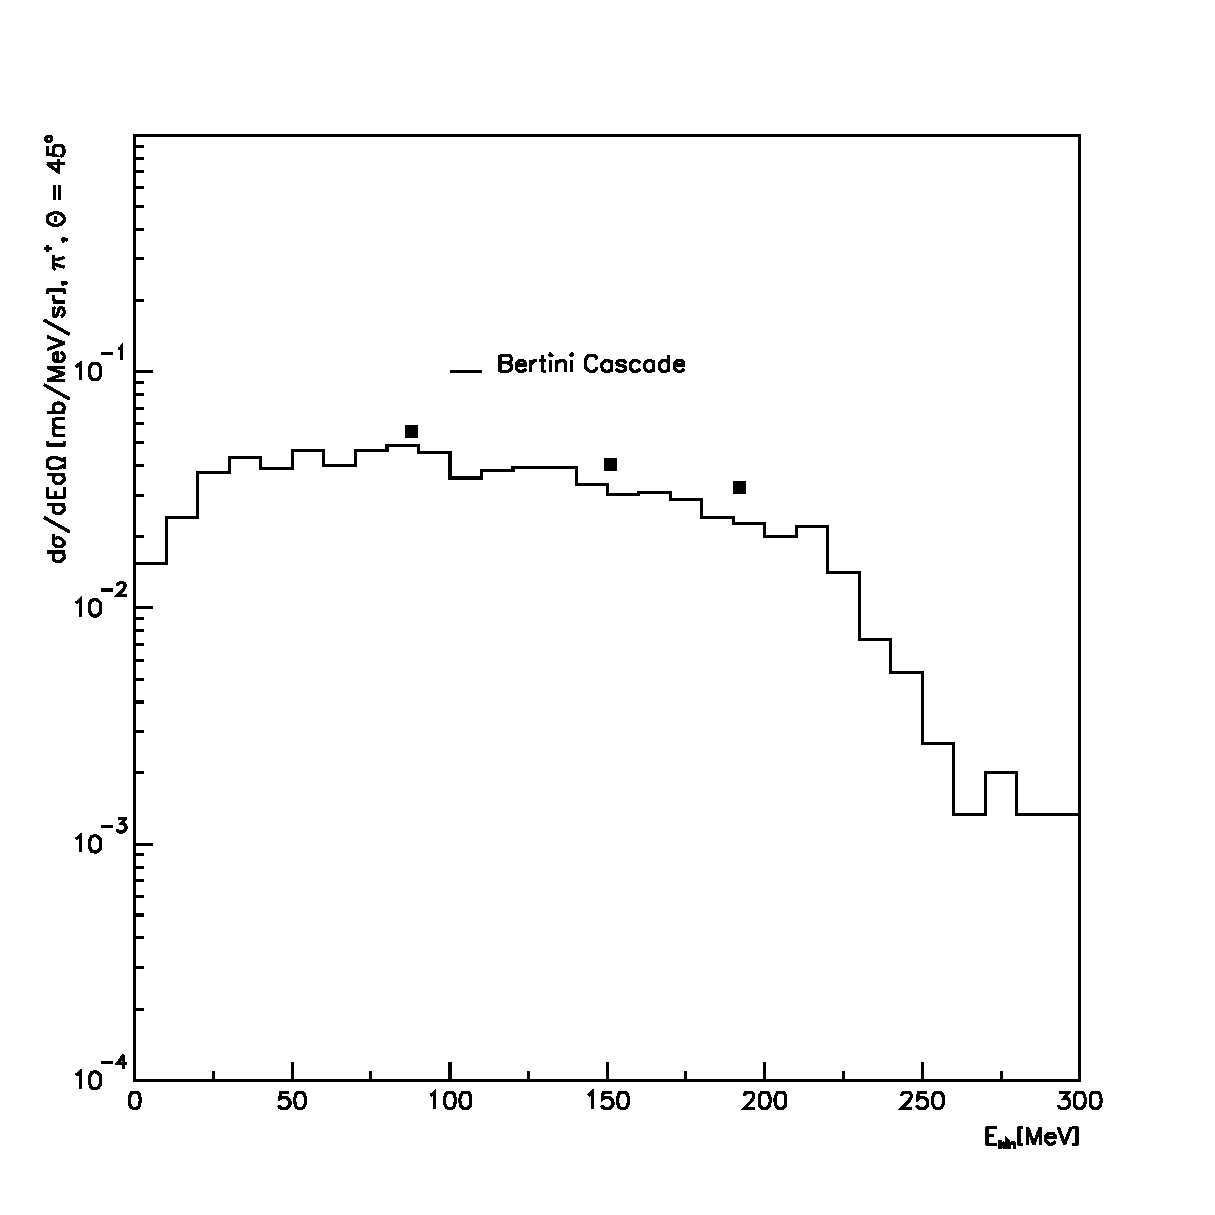
\includegraphics[width=80mm,keepaspectratio]{pn_pb_597_pip_a1.eps}
  \caption{$p(597 MeV)$ + Pb $\rightarrow$ $\pi^{+}(\theta = 45^{\circ})$ + X.}
  \label{pi45}
\end{figure}

\begin{figure}
  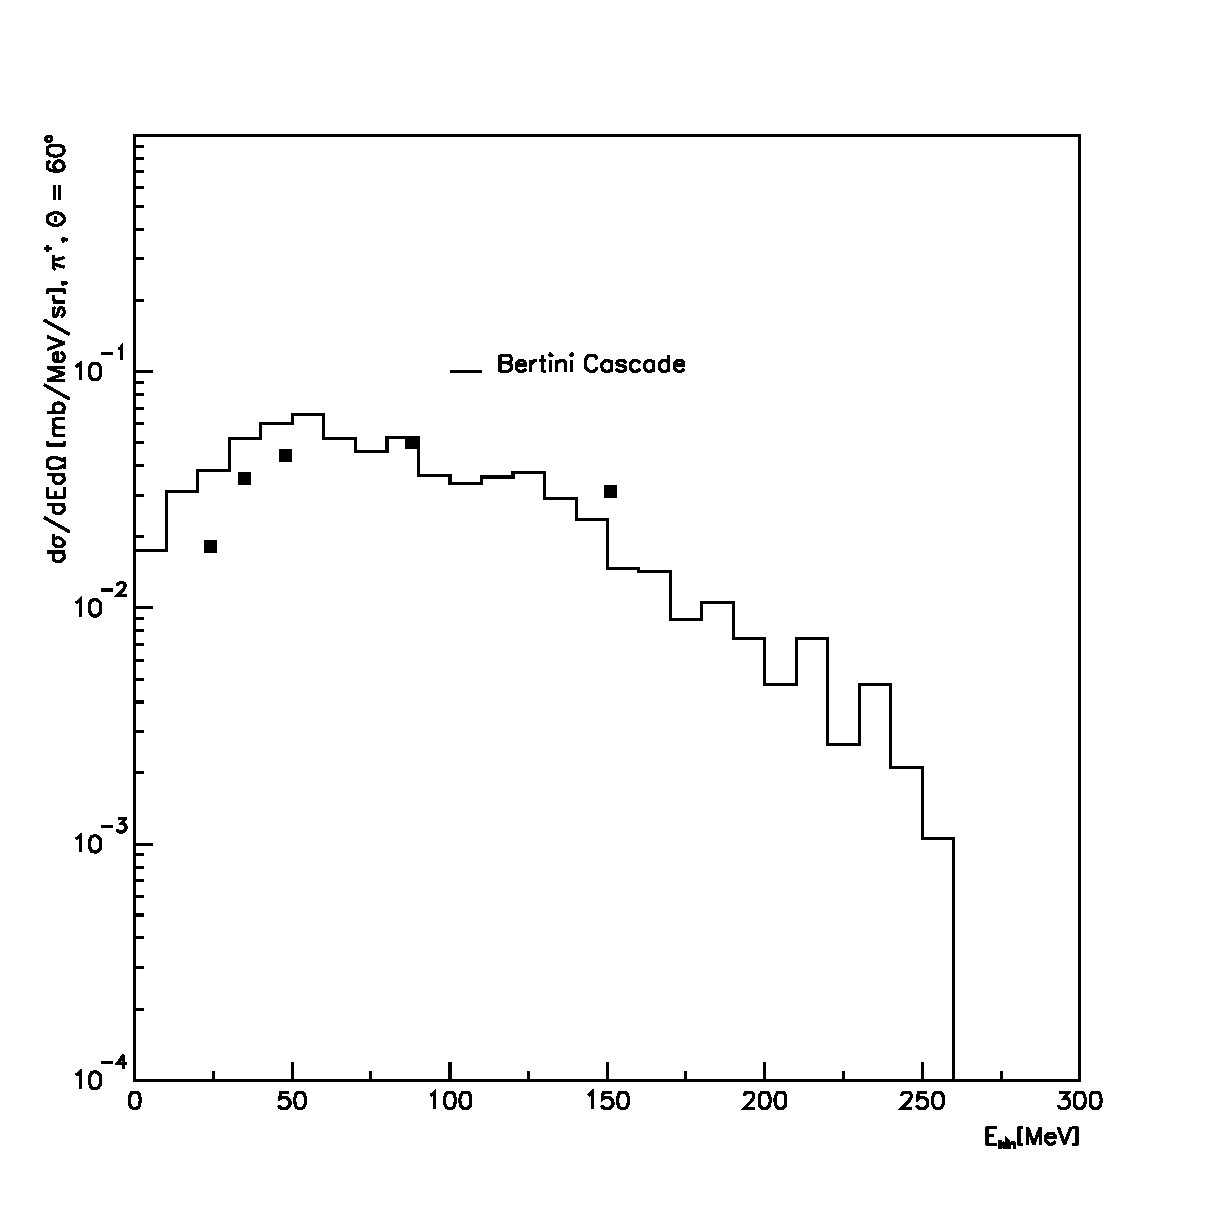
\includegraphics[width=80mm,keepaspectratio]{pn_pb_597_pip_a2.eps}
  \caption{$p(597 MeV)$ + Pb $\rightarrow$ $\pi^{+}(\theta = 60^{\circ})$ + X.}
  \label{pi60}
\end{figure}
 
\begin{figure}
  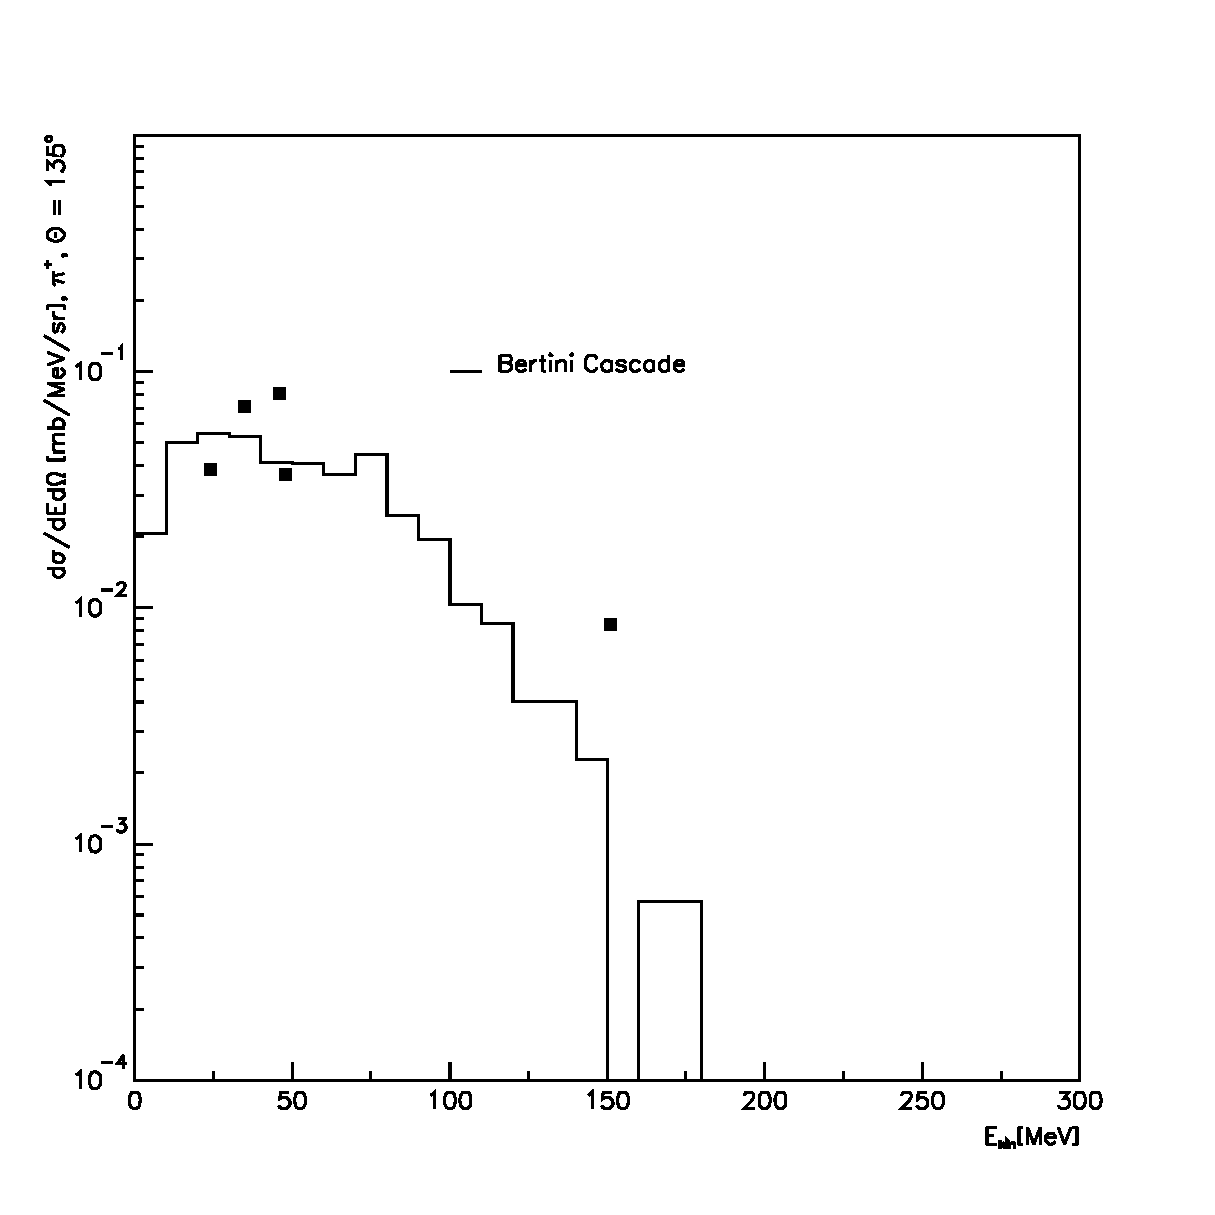
\includegraphics[width=80mm,keepaspectratio]{pn_pb_597_pip_a4.eps}
  \caption{$p(597 MeV)$ + Pb $\rightarrow$ $\pi^{+}(\theta = 135^{\circ})$ + X.}
  \label{pi135}
\end{figure}


\section{CONCLUSION}
We have released a Bertini INC model in Geant4.
Exitons, pre-equilibrium, nucleus explosion, fission, and evaporation are modelled.
Particles treated: $\gamma$, $\pi$, n, p, and nuclear isotopes 
We have tested the code in a energy range 60~MeV - 3~GeV and found a reasonable agreement with
experimental data. Tuning of performance and models are planned for future Geant4 releases.
Als, we plan to extend the upper energy limit of the models.
%\item Reasonable agreement with experimental data
%\item HETC nuclei model and other features will be incorporated later

 

%-----------------------

%\begin{acknowledgments}

%\end{acknowledgments}

%----------------------------< REFERENCES >----------------------------
%\bibliography{SiBTDAQ2002}
%\bibliography{/home/miheikki/public/html/system/references/references}

% Using the bib file will cause the reference numbers to be left out ?!


\begin{thebibliography}{9}

\bibitem{serber47}
R.~Serber, ``Nuclear Reactions at High Energies'',
Phys. Rev. 72, 1948

\bibitem{goldberger48}
M. Goldberger, ``The Interaction of High Energy Neutrons and Hevy Nuclei'',
Phys. Rev. 74, 1948

\bibitem{metropolis58}
N.~Metropolis et al., ``Monte Carlo Calculations on Intranuclear Cascades. I. Low-Energy Studies'',
Phys. Rev. 110, 1958

\bibitem{bertini68}
H.~W.~Bertini et al.,
Nucl. Instr. and Meth  66, 1968


\bibitem{bertini69}
H.~W.~Bertini, ``Intranuclear-{C}ascade {C}alculation of the {S}econdary {N}ucleon {S}pectra from {N}ucleon-{N}ucleus 
        {I}nteractions in the {E}nergy {R}ange 340 to 2900 {M}e{V} and {C}omparisons with {E}xperiment'',
Phys. Rev.  188, 1969


\bibitem{bertini71}
H.~W.~Bertini and P.~Guthrie, ``Results from Medium-Energy Intranuclear-Cascade Calculation'',
Nucl. Phys.  A169, 1971

\bibitem{alsmiller90}
R.~G.~Alsmiller, F.~S.~Alsmiller and O.~W.~Hermann, 
``The high-energy transport code HETC88 and comparisons with experimental data'',
Nucl. Instr. and Meth A295, 1990

\bibitem{titarenko99a}
Yu.~E.~Titarenko et al.,
``Experimental and Computer Simulations Study of
		  Radionuclide Production in Heavy Materials
		  Irradiated by Intermediate Energy Protons'',
nucl-ex/9908012, 1999

\bibitem{weisskopf37}
V.~Weisskopf,
``Statistics and {N}uclear {R}eactions'',
Phys. Rev. 52, 1937

\bibitem{dostrovsky59}
I.~Dostrovsky, Z.~Zraenkel and G.~Friedlander,
``Monte {C}arlo {C}alculations of {H}igh-{E}nergy {N}uclear {I}nteractions. {I}{I}{I}. 
{A}pplication to {L}ow-{E}nergy {C}alculations'',
Phys. Rev. 116, 1959

\bibitem{dostrovsky60}
I.~Dostrovsky, Z.~Zraenkel and P.~Rabinowitz,
``Monte Carlo Calculations of Nuclear Evaporation Processes. V. Emission of Particles Heavier Than $^4\!He$'',
Phys. Rev. 1960


\bibitem{griffin66}
J.~J.~Griffin,
``Statistical Model of Intermediate Structure'',
Phys. Rev. Letters 17, 9, 1966

\bibitem{geant4collaboration03}
Geant4 collaboration,
``Geant4 general paper'',
Nucl. Instr. and Meth A, 2003 (to be published)

\bibitem{letaw83}
J.~R.~Letaw et al.,
The Astrophysical Journal Supplements, 51, 1983


\bibitem{letaw93}
J.~R.~Letaw et al.,
The Astrophysical Journal, 414, 1993


\bibitem{pearlstein89}
S.~Pearlstein,
``Medium-energy nuclear data libraries: a case study, neutron- and proton-induced reactions in $^{56}${F}e'',
The Astrophysical Journal, 346, 1989

\bibitem{barashenkov72}
V.~S.~Barashenkov and V.~D.~Toneev,
``High Energy interactions of particles and nuclei with nuclei'',
(In russian), 1972

\bibitem{ribansky73}
I.~Ribansky et al.,
``Pre-equilibrium decay and the exiton model'',
Nucl. Phys. A203, 1973

\bibitem{kalbach78}
C. Kalbach,
``Exiton Number Dependence of the Griffin Model Two-Body Matrix Element'',
Z. Physik, A287, 1978


\bibitem{fong69}
P.~Fong,
``Statistical Theory of Fission'',
Gordon and Breach, New York, 1969

\bibitem{benchmarkData02}
[:::];

%strip detectors in a test beam'', . A453, 2000

\end{thebibliography}
%----------------------------< APPENDICES >----------------------------

\end{document}
%----------------------------< END OF FILE >---------------------------








%\begin{figure}
%  \begin{center}
%    \leavevmode
%    \mbox{\epsfxsize=13cm \epsffile{pictures/z001n002p001e000585c010h000.eps} }
%       \caption{ Geant4 simulation of proton with $585~MeV$ energy hitting deuterium atom $A(Z = 1,N = 2)$ 10000 times.}
%  \label{pic:z001n002p001e000585c010h000}
%  \end{center}
%\end{figure}



%    Date: Wed, 19 Mar 2003 18:31:45 +0100
%From: Hans-Peter Wellisch <Hans-Peter.Wellisch@cern.ch>
%To: Mika.Heikkinen@cern.ch
%Subject: Bertini cascade plots
% 
%Hi Aatos,
% 
%  I have made a set of plots, ands deposited them gere at CERN in
%~jwellisc/public/ForAatos
%There are  directories
% 
%pn_al_256
%pn_be_256
%pn_fe_256
%pn_pb_256
%pn_pb_597
% 
%that contain plots on proton induced neutron production (hence pn) on
%various materials (like be for Beryllium) at two difference energies
%(156MeV, 597MeV).
%The 597MeV directory in addition has pion production plots.
% 
%Many greetings,
% 
%Hans-Peter.            

%\begin{figure}
%  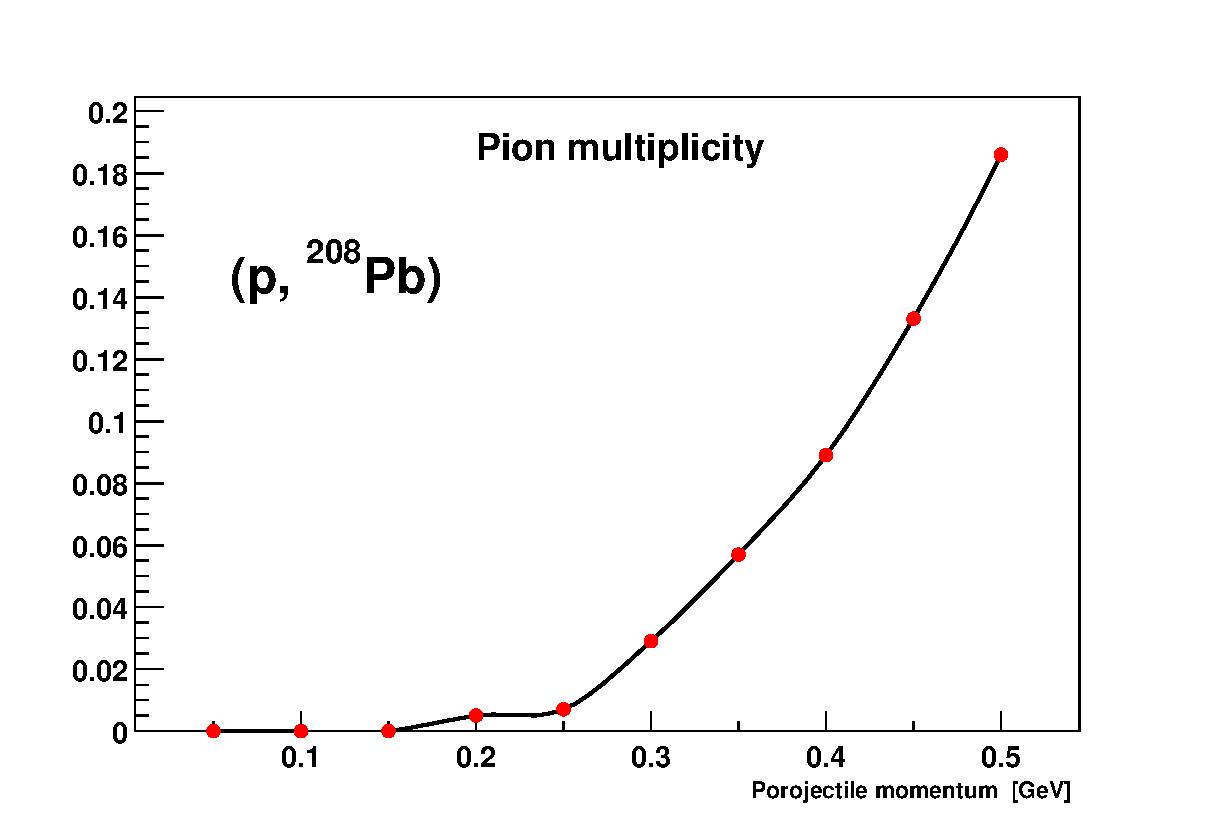
\includegraphics[width=80mm,keepaspectratio]{../pictures/pPbPionMultiplicity.eps}
%  \caption{Schematical layout of the SiBT experiment.}
%  \label{fig_mc}
%\end{figure}

%\begin{figure}
%  \includegraphics[width=80mm,keepaspectratio]{../pictures/resInuclPbIsotopes.eps}
%  \caption{Schematical layout of the SiBT experiment.}
%  \label{fig_mc}
%\end{figure}


%-----------------------


%\subsection{Introduction to Bertini INC}
%\begin{itemize}
%\item Physical justification: if the deBroglie wavelenght of the incident particle is 
%comparable to the average intra-nucleon distance, interactions can be treated in terms of 
%particle-particle collisions
%\item Condition of validity of the INC model:
%$\lambda_{B} / v << \tau_{c} << \Delta t$ \\

%$\delta_{B} = $ de Broglie wavelenth of the nucleons \\ 
%$v = $ average relative nucleon-nucleon velocity \\
%$\Delta t = $ time interval between collisions
%}
%\item Bertini INC solves the Boltzman equation on the average
%\item Physical foundation comes approximate if $E < 200~MeV$ or $E > 5~GeV$ 
%\item Pre-equilibrium model developed to support low energy treatment
%\end{itemize}
 

 
%\subsection{Basics of INC model steps}

%\begin{enumerate}
%\item The spatial point, where the incident particle enters, is selected uniformly over the projected area of the nucleus.
%\item Nucleon-nucleon cross-sections and region-depenent nucleon densities 
%are used to select a path lenght for the projectile particle.
%\item The momentum of the struck nucleon, the type of reaction 
%and four momentum of the reaction products are determined.
%\item Exiton model is updated as the cascade proceeds.
%\item If Pauli exclusion principle allows and
% $E_{particle} > E_{cutoff} = 2~MeV$, step (2) is performed to transport the products.
%\end{enumerate}
 


 
%\subsection{Nuclei model}%

%\begin{itemize}
%\item Three concentric spheres. 
%\item Impulse distribution in each region of concentric spheres follows
% Fermi distribution with zero temperature
%\item Pauli exclusion principle (crosses) is taken into account by accepting only secondary nucleons with
% $E_N > E_{Fermi}$
%\end{itemize}

%\begin{figure}
%  \includegraphics[width=80mm,keepaspectratio]{../pictures/mc.eps}
%  \caption{Schematical layout of the SiBT experiment.}
%  \label{fig_mc}
%\end{figure}


 
%\subsection{Cross-sections}

%\begin{itemize}
%\item Path lengths of nucleons in the nucleus are sampled according to the local density and to
% free nucleon-nucleon cross-sections
%\item Angles after collisions are sampled from experimental differential cross-sections
%\item Tabulated total reaction cross-sections are calculated by Letaw's formulation
%\item For pions the INC cross-sections are provided to treat elastic collisions and inelastics channels
%($\pi^{0}$p $\rightarrow$ $\pi^{+}$n etc.)
%\item Pion absorption channels 
%($\pi^{+}$nn $\rightarrow$ pn  etc.)
%\item Multiple particle production is also implemented
%\end{itemize}
 


 
%\subsection{Pre-equilibrium model}

%\begin{itemize}
%\item Implements exiton model proposed by Griffin
%\item Nucleon states are characterized by the number of exited particles and holes
% (the exiton model proposed by Griffin)
%\item INC collisions give rise to a sequence of states characterized by increasing exciton number, 
%leading to a equilibrated nucleus
%\item In exiton model the posible selection rules for a particle-hole configuarations in the cource of the cascade are:
%$\Delta p = 0, \pm 1$  $\Delta h = 0, \pm 1$  $\Delta n = 0, \pm 2$,
%where p is the number of particle, h is number of holes and n = p + h is the number of exitons. 
%\item The angular distribution is isotropic in the frame of rest of the exiton system.
%\item Parametrisations of the level density  (tabulated with both A and Z dependence)
%behaviour (the nuclei binding energy using smooth liquid high energy formula).
%\end{itemize}
 

 
%\subsection{Break-up models}
%
%\begin{itemize}
%\item Fermi break-up is allowed in extreme cases (if $A < 12$ and
%  $3 (A - Z) < Z < 6$ or if $E_{exitation} > 3 E_{binding}$) 
%\item Simple explosion model decreases exotic evaporation processes
%\item Phenomenological fission model uses potential minimization
% (incorporating binding energy paramerization and fission statistical model features)
%\end{itemize}
 

 
%\subsection{Evaporation model}
%\begin{itemize}
%\item Statistical theory for particle emission of the exited
% nucleus remaining after the INC (by Weisskopf)
%%\item This model assumes complete energy equilibration before the particle emission, 
%and re-equilibration of excitation energies between successive evaporations. 
%\item As a result the angular distribution of emitted particles is isotropic.

%\item Geant4 evaporation model for cascade implementation adapts often used computational method developed by Dostrowski
%\item The emission of particles is computed until the exitation energy fall below some spesific cutoff
%\item If light nucleus is higly exited Fermi break-up model is executed. Also, fission is performed if channel is open
%\item The main chain of evaporation
%(followed until  E$_{cutoff}$ = 0.1 MeV) 
%\item The evaporation model ends with  $\gamma$ emission chain (followed until 
%E$^{\gamma}_{cutoff}$ = 10$^{-15}$ MeV)
%\end{itemize}
 

 
%\subsection{Geant4 implementation}
%\begin{itemize}
%\item Bertini INC is based on re-engineering of INUCL fortran code
%\item C++ version INUCL++ is a compact stand alone code
%\item Implemented in Geant4 hadronics physics framework, 
%which allows modular implementation  
%%various kinds of hadronic interactions
%\item Source code in {\it processes/\-hadronic/\-models/\-cascade/\-cascade}
%\item 16K lines in 32 classes (4K lines for testing and documentation)
%\end{itemize}
 



 
%\subsection{Interfacing Bertini INC models}
%\begin{itemize}
%\item Current implementation is quite loosely connected to the Geant4 hadronic framework
%\item Models are organised into separate classes  
%({\it G4IntraNucleiCascader, G4Fissioner, G4NonEquilibriumEvaporator, G4EquilibriumEvaporator} etc.)
%\item All the models are used collectively through interface method 
%{\it Apply\-Yourself} defined in a class {\it G4Cascade\-Inteface}
%\end{itemize}
 


% 
%\setlength{\epsfxsize}{0.6\textwidth} \epsffile{pictures/ForAatos/pn_al_256/n_a.eps}

%{\small \it :::.}
% 
%--------------
% 
%\setlength{\epsfxsize}{0.6\textwidth} \epsffile{pictures/ForAatos/pn_al_256/n_a0.eps}
%
%{\small  $p^{256 MeV}$ + Al $\rightarrow$ $n^{\theta = 7.5^{\circ}}$ + X}
%{\small \it 256 MeV proton induced neutron production ($\theta = 7.5^{\circ}$) in Al}
% 
%
% 
%\setlength{\epsfxsize}{0.6\textwidth} \epsffile{pictures/ForAatos/pn_al_256/n_a1.eps}
%
%{\small  $p^{256 MeV}$ + Al $\rightarrow$ $n^{\theta = 30^{\circ}}$ + X}
% 
%
% 
%\setlength{\epsfxsize}{0.6\textwidth} \epsffile{pictures/ForAatos/pn_al_256/n_a2.eps}
%
%{\small  $p^{256 MeV}$ + Al $\rightarrow$ $n^{\theta = 60^{\circ}}$ + X}
% 

% 
%\setlength{\epsfxsize}{0.6\textwidth} \epsffile{pictures/ForAatos/pn_al_256/n_a3.eps}
%
%{\small \it Proton induced neutron production in aluminium at 256 MeV.}
% 

% 
%\setlength{\epsfxsize}{0.6\textwidth} \epsffile{pictures/ForAatos/pn_al_256/n_a4.eps}
%
%{\small  $p^{256 MeV}$ + Al $\rightarrow$ $n^{\theta = 150^{\circ}}$ + X}
% 

%-----------------


% 
%\setlength{\epsfxsize}{0.6\textwidth} \epsffile{pictures/ForAatos/pn_be_256/n_a0.eps}
%
%{\small  $p^{256 MeV}$ + Be $\rightarrow$ $n^{\theta = 7.5^{\circ}}$ + X}
% 
%
% 
%\setlength{\epsfxsize}{0.6\textwidth} \epsffile{pictures/ForAatos/pn_be_256/n_a1.eps}
%
%{\small  $p^{256 MeV}$ + Be $\rightarrow$ $n^{\theta = 30^{\circ}}$ + X}
% 
%
% 
%\setlength{\epsfxsize}{0.6\textwidth} \epsffile{pictures/ForAatos/pn_be_256/n_a2.eps}
%
%{\small  $p^{256 MeV}$ + Be $\rightarrow$ $n^{\theta = 60^{\circ}}$ + X}
% 
%
% 
%\setlength{\epsfxsize}{0.6\textwidth} \epsffile{pictures/ForAatos/pn_be_256/n_a3.eps}
%
%{\small \it Proton induced neutron production in beryllium at 256 MeV.}
% 
%
% 
%\setlength{\epsfxsize}{0.6\textwidth} \epsffile{pictures/ForAatos/pn_be_256/n_a4.eps}
%
%{\small  $p^{256 MeV}$ + Be $\rightarrow$ $n^{\theta = 150^{\circ}}$ + X}
% 

%---------------------
